\chapter{Fonctionnalité implémentées}

\section{Les annotations}

Plusieurs annotations différentes à ajouter aux vidéos ont été implémentées. Si l'on lance le traitement les choix d'annotations se font seulement avant le lancement du programme dans le fichier annotation\_settings.json.
Si on lance l'interface, les choix d'affichage s'initialisent grâce au fichier Json mais peuvent changer au cours de la vidéo. 
Nous allons donc suivre l'architecture du fichier Json pour expliquer les différentes fonctionnalités implémentées pour les annotations.
\bigskip

Le booléen write présent pour chaque annotation exprime l'écriture ou non sur l'image de l'annotation.
\bigskip



\subsection{Les couleurs}

Les deux premiers éléments du fichier json sont les couleurs des équipes. Par défaut, les couleurs des équipes sont bleu pour l'équipe 1 et rose pour l'équipe 2, ce qui correspond aux couleurs des robots en match.

Il faut également récupérer les numéros des équipes. Soit ils sont connus, soit il faut les récupérer avec le l'exécutable init\_match.

\subsection{La position}

La position permet d'afficher un cercle montrant la position où le robot pense être.
Elle s'affiche forcément pour tous les robots à la fois ou aucun. Il est possible de choisir le rayon du cercle (en pixel) et l'affichage ou non du numéro du robot au centre de la position. 
\bigskip

La taille de l'écriture du numéro est proportionnelle au 3/4 du rayon du cercle, il est donc inutile de l'afficher si la taille est minime.

La position s'affiche simplement en transformer le point du plan en point sur l'image grâce à la fonction fieldToImg fournie par le client.

\subsection{La direction}

Tout comme la position, l'annotation de la direction dessine une flèche montrant la direction dans laquelle le robot avance. Il est possible de changer la taille de cette flèche.
\bigskip

La flèche est créée en définissant un second point sur le dessin dans la direction donnée (en radian). Ce point est trouvé en additionnant les coordonnées de la position à $\cos$(direction) pour l'axe des $x$ et $\sin$(direction) pour l'axe des  $y$.

Ensuite, nous transposons nos deux points dans le plan de l'image grâce à fieldToImg.

Enfin, nous calculons la distance entre ce nouveau point et la position grâce au théorème de Pythagore puis nous réduisons proportionnellement cette distance à la taille de la flèche souhaitée.
\bigskip

Nous affichons la flèche de la couleur de l'équipe du robot. Il se peut que la flèche s'affiche en noir, cela signifie que l'angle donné par le robot est supérieur $2*\Pi$ et donc qu'il y a sûrement une imprécision du robot. 
Nous pouvons voir cette erreur dans la vidéo 2vs1.


\subsection{La trace}

L'annotation de la trace est représentée par de multiples cercles représentant les anciennes positions du robot. 
La trace ne peut être visible que sur un robot à la fois, il peut être changé en cours de match lorsque la visualisation est lancée avec l'interface. 
\bigskip

Elle s'affiche de la même couleur de l'équipe mais en plus foncé comme on peut le voir dans la Figure~\ref{fig:trace}.
Nous pouvons choisir la taille de la trace, il est préférable de l'avoir plus petit que la position.


La trace nous montre les dernières positions depuis un certain nombre de secondes définit dans delay\_old\_pos. La trace est stockée dans une map.
\bigskip
Pour afficher la trace nous affichons donc toutes les positions présentes dans la map pour un certain nombre de seconde précèdent.


\begin{figure}[h] 
\centering 
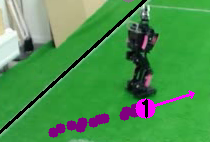
\includegraphics[scale = 0.5]{images/robottrace.png}
    \caption{Affichage de la trace}
    \label{fig:trace}
\end{figure}

Nous avons un problème majeur sur la trace qui est le stockage des données. En effet, nous stockons les positions dans une map définie par les time\_stamp des positions. 

Nous avons essayé de faire un pointeur sur l'objet du robot mais la suppression des messages n'est jamais prise en compte et donc à chaque fois que nous appelons l'annotation de la trace nous récupérons seulement les positions intéressantes sans jamais en supprimer. 

L'avantage est donc que lorsque l'on se déplace dans la vidéo avec l'interface, si nous revenons dans des moments déjà visités, la trace s'affiche sur le délai voulu et sans problème.

\subsection{La balle}

Tout comme la trace, nous ne pouvons voir la balle du point de vue d'un seul robot à la fois. Nous pouvons choisir la taille de la balle. La couleur de la balle est définie arbitrairement en gris.
\bigskip

Ce qui a été compliqué avec la balle c'est que la position de la balle est donnée dans le repère du robot, non du terrain. 

En effet, dans les logs Figure~\ref{fig:message}, la position du robot est définie grâce self\_in\_field donc dans le repère du terrain mais la position de la balle est dans ball\_in\_self donc d'après le repère du robot.
\bigskip

Nous avons donc du changer de repère grâce à une équation de plan.

Soit ($x_B$, $y_B$) les coordonnées de la balle dans le repère du robot et ($x_B$',$y_B$') dans le repère du terrain. On définit également ($x_R$, $y_R$) les coordonnées du robot dans le plan du terrain et $\theta$ l'angle de la direction du robot en radian. L'équation est donc :

\[\left\{
  \begin{array}{ccccccc}
    x_B'& =& x_R &+& x_B \cos(\theta)& - & y_B \sin(\theta)\\
    y_B' &= & x_R &+& x_B \sin(\theta)& +& y_b \cos(\theta)\\
  \end{array}
\right.
\]    

\subsection{La position souhaitée (Target)}

La target représente la position que le robot souhaite atteindre. Elle ne s'affiche donc que pour un robot à la fois.
\bigskip

Elle est marquée par une croix dont la taille est définie par l'utilisateur dans target\_size. Si on a également la position du robot, une ligne en pointillé s'affiche entre la position du robot et celle souhaitée. 
Il est possible de ne pas afficher cette ligne en mettant un nombre plus grand que la taille de l'image (avec les vidéos données, 1000 convient parfaitement).
\bigskip

La taille des traits est égale à la taille des espaces, pour tracer la ligne, nous avons fait un itérateur qui colorise un certain nombre de pixel pour le trait puis qui laisse l'espace de même taille.

\begin{figure}[h] 
\centering 
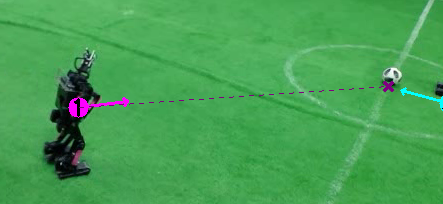
\includegraphics[scale = 0.5]{images/robottarget.png}
    \caption{Affichage de la target}
    \label{fig:target}
\end{figure}

\subsection{Les lignes du terrain et le score}

Nous pouvons choisir d'afficher les lignes du terrain en fournissant le fichier Json définissant les caractéristiques du terrain sur lequel le match est joué. 
Ce fichier Json est nécessaire pour la calibration de la caméra.
\bigskip

Comme nous en avons vu Figure~\ref{fig:field} à la page~\pageref{fig:field}, les lignes du terrain peuvent parfois avoir des erreurs à cause de la distorsion de la caméra.
Afficher ces lignes peut nous aider à comprendre les différences entre la position annotée et réelle du robot.
\bigskip

Il y a une possibilité d'afficher le score dans un des coins de l'écran. Les valeurs à donner en x et y sont données en commentaire dans le Json. Nous n'avons pas défini de coin par défaut car il peut changer à chaque vidéo. Par exemple, l'idéal pour la vidéo static de 2vs1 est dans le coin en haut à gauche mais si on l'affiche là, le score ne se voit pas sur la vidéo webcam du 21/03/2019.
\bigskip

Il faut noter que le score s'affiche automatiquement dans l'interface.

\subsection{Délai et optimisation des annotations}

Les deux derniers éléments du fichier Json sont delay\_annotation et optimized. Le premier exprime le temps en seconde durant lequel un message est considéré comme valide. C'est à dire le temps pour lequel on va l'afficher avant qu'il soit trop vieux.
\bigskip

L'optimisation permet d'afficher les annotations avec une opacité reflétant la durée. Un message plus vieux sera plus transparent qu'un message tout juste reçu. 
\bigskip

Pour l'ajout de certaines annotations comme la trace, nous avons souhaité utiliser la transparence.
Ainsi, les anciennes positions deviennent graduellement transparentes, jusqu'à disparaître.


\begin{figure}[h] 
\centering 
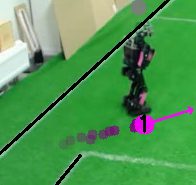
\includegraphics[scale = 0.5]{images/traceoptimized.png}
    \caption{Affichage de la trace optimisé}
    \label{fig:trace_opti}
\end{figure}


Malheureusement, les fonctions de dessin d'OpenCV ne gèrent pas la transparence.
OpenCV gère bien les images avec transparence, les fonctions de dessin acceptent des couleurs avec transparence, mais lors du dessin, elles ignorent cette valeur et dessinent en pleine opacité. 
\bigskip

Nous avons donc décidé d'utiliser la fonction d'OpenCV (AddWeighted) permettant de fusionner deux images en fonction d'une opacité.
\bigskip

La transparence des objets se fait en trois étapes.

Tout d'abord, on calcule l'opacité en fonction du temps. Ensuite on copie l'image dans une image provisoire (overlay) et on ajoute l'annotation à cette copie. Ensuite on ajoute l'image copiée et annotée à l'image de départ (blend) en fonction de l'opacité calculée grâce à la fonction OpenCV. 
\bigskip

La différence de performance entre les annotations non optimisées et optimisées est calculée dans les tests sur la performance.

\section{Le traitement}

En dehors des tests, nous avons deux fichiers exécutables dans la partie du traitement.

\subsection{Init\_match}


Tous les choix sur les numéros de robot et d'équipe peuvent être difficiles si on ne connaît pas les robots de la vidéo. 
L'exécutable init\_match permet de lire les 30 premières secondes de vidéo et de connaître donc les robots présent en jeu ainsi que leur équipe. On peut en voir le résultat Figure~\ref{fig:init_match} :

\begin{figure}[h] 
\centering 
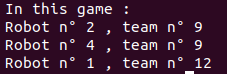
\includegraphics[scale = 0.5]{images/init_match.png}
    \caption{Résultat de l'exécutable init\_match}
    \label{fig:init_match}
\end{figure}


Tout comme les tests, il faut activer les tools de traitement dans le CMakeList pour avoir l'exécutable init\_match.

\subsection{Main\_Traitement}

Notre fichier principal de lancement est l'outil main\_traitement.
Il permet de lancer un monitoring et d'afficher une vidéo simplement, comme cela a été détaillé dans l'architecture du projet.
\bigskip

Il y a une option ajustable pour le fichier main\_traitement dans le fichier de configuration match\_settings. Il s'agit de l'élément speed\_optimized. Si, l'utilisateur met ce booléen à false, alors le match défilera le plus vite possible pour l'ordinateur.
Sinon, le match défilera à vitesse normale, c'est à dire à la même vitesse que le fichier vidéo fourni.
\bigskip

Pour cela, nous calculons le temps réel écoulé depuis le lancement de la vidéo grâce à deux chronos. Nous comparons ensuite ce temps écoulé au temps écoulé de la vidéo.
\bigskip

Si nous avons de l'avance par rapport à la vidéo alors nous ralentissons grâce à un temps d'attente avant la prochaine image. 
Sinon nous passons immédiatement à l'image suivante. En cas de retard trop important, nous sautons une image ce qui nous permet de ne pas avoir de retard par rapport à la vidéo.

\section{L'interface}


Nous ajoutons des annotations sur une vidéo de match. Cependant, étant donné le grand nombre d'informations, l'image peut se trouver saturée et devenir illisible. Notre interface doit résoudre ce problème en proposant des options d'affichage qui conviennent à différents usages.
\bigskip

\subsection{Choix de l'API}

Dans un premier temps, il a fallu choisir une API pour créer l'interface de notre programme. Nous en cherchions une plutôt facile à prendre en main, en c++, et qui propose suffisamment d'options pour créer une interface complète. 
\bigskip

Nous avons d'abord pensé à openCV, que nous utilisons déjà abondamment pour les annotations. La prise en main est assez rapide mais les options sont trop peu nombreuses. Les interfaces en openCV se limitent principalement à afficher des images, sans trop de fioritures. 
\bigskip

GTK et FLTK ont été rapidement considérés, mais la prise en main semblait trop compliquée et aurait pris trop de temps. 
\bigskip

Nous avons donc choisit QT dans sa version 5.9, qui est très bien documenté, facile à prendre en main et présente un très large éventail d'options pour créer une interface riche et complète.
\bigskip

Au début du projet, nous avons rencontré des difficultés pour faire communiquer l'interface et les fonctions d'annotation. Après la refonte de l'architecture du projet, la liaison entre les modules interfaces et traitement était grandement simplifiée, et nous avons pu lire une vidéo dans notre fenêtre QT. 
\bigskip

Nous avons ensuite pu ajouter des options pour choisir les annotations à afficher, modifiables pendant la lecture de la vidéo. 
\bigskip

De chaque coté de la vidéo, nous affichons des informations sur le déroulement du match, les robots et les équipes.
\bigskip

\subsection{Le slider}

Un slider a été implémenté pour choisir un moment précis de la vidéo. Il s'agit d'un slider prenant des valeurs de 0 à 99. Lorsque le slider est déplacé par l'utilisateur, nous utilisons le nombre total d'images de la vidéo et la lecture reprend au pourcentage de vidéo correspondant à la valeur du slider. 
\bigskip

Pour que le slider avance automatiquement lorsque la vidéo est en lecture, nous comptons le nombre d'images, et en le divisant par le nombre total d'image (et en multipliant par 100), nous obtenons la valeur à laquelle placer le curseur du slider. 
\bigskip

Lorsque le slider est déplacé, le time\_stamp correspondant à l'image et aux messages à lire est incrémenté (respectivement décrémenté) jusqu'à atteindre la position indiquée par le slider. Seul un entier est modifié dans une boucle while, nous ne parcourons pas toutes les images entre les deux time\_stamp. 
\bigskip

On affiche le temps écoulé dans un label en dessous du slider. Ce temps est exprimé en minutes et secondes. Les matchs ne devraient pas durer une heure, notamment à cause de la batterie des robots. Il nous a semblé plus pertinent de simplifier l'affichage en ayant seulement deux nombres (minutes et secondes) plutôt qu'un nombre pour les heures qui serait égal à 0 dans la majorité des cas. Si le match dure plus de 60 minutes, le nombre de minute continuera d'incrémenter. 
\bigskip

\subsection{Interface Débug}
Cette interface est celle qui propose le plus d'options. L'utilisateur choisit quelles annotations seront affichées et pour quel(s) robot(s). 
\bigskip

Pour alléger l'interface, la sélection des éléments à afficher se fait dans une fenêtre surgissante [Pop-up]. L'utilisateur coche les annotations qui l'intéressent, valide, puis choisit les robots sur la fenêtre principale. Le changement prend effet dès l'image suivante.  
